\documentclass[a4paper,12 pt]{report}
\usepackage{latexsym}
\usepackage[utf8]{inputenc}


%\usepackage[english]{babel}
\usepackage[italian]{babel}
% Per cambiare la parola listing con Codice
\addto\captionsitalian{\renewcommand{\lstlistingname}{Codice}}



\usepackage{makecell}
\usepackage{tabstackengine}
\usepackage[table]{xcolor}
\usepackage{array}
\usepackage{graphicx}
\usepackage{makecell}
\usepackage{array, multirow}
\usepackage[table]{xcolor}
\usepackage{tabularx, tabulary, tabu, longtable}

\usepackage{svg}

\usepackage{graphicx}
\usepackage{hyperref}
\usepackage[table,xcdraw]{xcolor}
\usepackage{setspace}
\usepackage{amssymb}
\usepackage{listings}
\usepackage{url}

\usepackage{xcolor}
\usepackage[T1]{fontenc}
\newcommand\myworries[1]{\textcolor{red}{#1}}

\usepackage{enumitem}
\usepackage{float}
\usepackage{hyperref}
\usepackage{tikz}
\usepackage{multirow}
\usepackage{todonotes}
\usepackage{amsmath}
\usepackage{placeins}

\usepackage{amsthm}

\usepackage{graphicx}  
\usepackage{array}
\usepackage{booktabs} 
\usepackage{pifont}
\newcommand{\xmark}{\ding{55}}
\newcommand{\cmark}{\ding{51}} 

\usepackage[square,numbers]{natbib}

% package italiano
%
% Opzionale
%
% \renewcommand{\contentsname}{Sommario}
% \renewcommand{\listfigurename}{List of Figures}
% \renewcommand{\listtablename}{List of Tables}
% \renewcommand{\bibname}{Bibliografia}
% \renewcommand{\indexname}{Indice}
% \renewcommand{\figurename}{Figura}
% \renewcommand{\tablename}{Tavola}
% \renewcommand{\partname}{Parte}
% \renewcommand{\chaptername}{Capitolo}
% \renewcommand{\appendixname}{Appendice}
% \renewcommand{\abstractname}{Abstract}
% \renewcommand{\footnotesize}{\scriptsize}
% \renewcommand{\today}{\ifcase\month\or
%  Gennaio\or Febbraio\or Marzo\or Aprile\or Maggio\or Giugno\or
%  Luglio\or Agosto\or Settembre\or Ottobre\or Novembre\or Dicembre\fi
%  \space\number\day, \number\year}

% package formato
\pagestyle{plain}
\setlength{\topmargin}{0.0in}
\setlength{\headheight}{0.2in}
\setlength{\headsep}{0.0in}
\setlength{\footskip}{0.5in}
\setlength{\textheight}{8.3in}
\setlength{\textwidth}{6.0in}
\setlength{\oddsidemargin}{0.5in}
\setlength{\evensidemargin}{0.5in}
\setlength{\parindent}{0.4 in}
\onehalfspacing


\def\cent{\centerline}
\def\vs{\vskip 10 pt plus 1 pt}
\def\bs{\bf}
\def\grad{\vec{\nabla}}
\def\gradx{\vec{\nabla}_x}
\def\epsilon{\varepsilon}

\newtheorem{theorem}{Theorem}[section]
\newtheorem{corollary}{Corollary}[theorem]
\newtheorem{lemma}[theorem]{Lemma}

\newtheorem{lemm}{Lemma}[chapter]
\newtheorem{proposizion}[lemm]{Proposizione}
\newtheorem{teorem}[lemm]{Teorema}
\newtheorem{corollari}[lemm]{Corollario}
\newtheorem{esempi}[lemm]{Esempio}

\newcommand{\cvd}{\begin{flushright}$\Box$\end{flushright}}
\newcommand{\tr}{{\rm Tr}\;}
\newcommand{\eq}{\begin{equation}}
\newcommand{\feq}{\end{equation}}
\theoremstyle{definition}
\newtheorem{definition}{Definition}[section]
 
\theoremstyle{remark}
\newtheorem*{remark}{Remark}

\definecolor{blu_dmi}{HTML}{002e62}


%%%%%%%%%%%%%%%%%%%%%%%%%%%%%%%%%
%%%%%%%%%%%%%%%%%%%%%%%%%%%%%%%%%
%%%%%%%%%%%%%%%%%%%%%%%%%%%%%%%%%
%%%%%%%%%%%%%%%%%%%%%%%%%%%%%%%%%



\begin{document}
    % Thesis frontmatter --------------------------------------------
\thispagestyle{empty} %suppress page number

	\noindent % just to prevent indentation narrowing the line width for this line
	
\includegraphics[width=0.15\textwidth]{img/logoUniPg}
	\begin{minipage}[b]{0.7\textwidth}
		\centering
		{\Large \textcolor{blu_dmi}{\textsc{Universit{\`a} di Perugia}}}\\
		\vspace{0.4 em}
		{\large \textcolor{blu_dmi}{Dipartimento di Matematica e Informatica}}
		\vspace{0.6 em}
	\end{minipage}%
	
\includegraphics[width=0.15\textwidth]{img/logoDMI}
	
	\vspace{5 em}

	\begin{center}
		
		{\large \textcolor{blu_dmi}{\textsc{Tesi triennale/magistrale in ...}}}
		\vspace{8 em}
		
		{\Huge \textcolor{blu_dmi}{Titolo Tesi}}
		\vspace{10 em}
		
		\makebox[380pt][c]{\textcolor{blu_dmi}{\textit{Advisor} \hfill \textit{Candidate}}}
		\makebox[380pt][c]{\textcolor{blu_dmi}{\textbf{Prof. Tizio \hfill  Caio}}}
%		\makebox[380pt][c]{\textcolor{blu_dmi}{\textit{Advisor} \hfill \textit{}}}
%		\makebox[380pt][c]{\textcolor{blu_dmi}{\textbf{Dott. Francesco Santini \hfill}}}
		
		\vspace{6 em}
		\vfill
		
		\textcolor{blu_dmi}{\rule{380pt}{.4pt}}\\
		\vspace{1.2 em}
		\large{\textcolor{blu_dmi}{Academic Year 2018-2019}}
		
		
		
		
	\end{center}

% ------------------------------------------------------------------
      \newpage 
  
  {%\clearpage           % we want a new page          %% I commented this
   \thispagestyle{empty}% no header and footer
   \vspace*{\stretch{1}}% some space at the top
   \itshape             % the text is in italics
   \raggedleft          % flush to the right margin
  }
  \begin{flushright}
  
    Alle mie nonne,
e in particolare alla pazienza di una di loro.
  
  
  \end{flushright}
  {\par % end the paragraph
   \vspace{\stretch{3}} % space at bottom is three times that at the top
   \clearpage           % finish off the page
  }

\newpage



    % Opzionale
    % \thispagestyle{empty} %suppress page number

\centerline{\emph{Sommario}}


\newpage

    
    \tableofcontents

    \chapter{Introduzione al DDS}
In questo capitolo viene fatta un'introduzione generale dello 
standard del Data Distribution Service (DDS) gestita
dall'Object Management Group (OMG). Inizialmente a livello generale 
per poi andare sempre più nel
dettaglio per capire il suo funzionamento, che ci sarà utile 
capire per comprendere le vulnerabilità che verranno analizzate in
successivi capitoli. Inoltre verrà introdotta la sua estensione
DDS security che si occupa di rendere più sicuro lo standard DDS 
aggiungendo elementi di sicurezza come l'autenticazione e una 
implementazione della cifratura dei pacchetti scambiati tra i vari
dispositivi connessi alla rete. Successivamente verranno mostrate delle 
implementazioni e in quali contesti viene utilizzato utilizzato
attualmente e in futuro. 
Infine verra mostrato in quali contesti attuali e futuri viene
utilizzato con le sue diverse implementazioni.

In questa tesi, in dei casi, verrà omessa la specifica OMG perchè 
ci riferiremo
esclusivamente al DDS conforme all'Object Management Group. Questo 
standard ha delle specifiche tecniche ben precise, consente
l'interoperabilità tra i diversi vendor che lo rispettano, insieme
a tanti altri numerosi vantaggi.
\cite{dds1.4}


\section{Modello publish/subscribe}
Prima di paralare del DDS, é necessario prima capire il 
funzionamento del modello Publish-Subscribe 
che sta alla base di tutto il suo funzionamento.
Questo sistema di publish e subscribe non funziona come la 
classica applicazione che siamo abituati a vedere tra server e
client tramite protocollo TCP/IP nell'ambito delle comunicazioni. 


\subsection{Perché non usiamo una connessione con TCP/IP}
Prendiamo l'esempio di un collegamento tra una workstation e 
un sensore per la temperatura. La connessione a livello fisico
avverrá tramite un collegamento Ethernet. La workstation e il 
sensore quindi si trovano nello stesso network e possono 
ora cominciare a comunicare tra di loro. L'obiettivo é quello
di trasferire i dati dal sensore alla workstation in modo tale
da poterli visualizzare a schermo.
Il metodologia piú frequente é quella di utilizzare un socket tramite 
protocollo TCP/IP, ma non sempre é la soluzione migliore.
Dei vantaggi del TCP/IP sono la disponibilitá di utilizzo 
in molte situazioni e nella maggior parte delle connessioni a 
Internet viene utilizzato questo protocollo.
Tuttavia, in certe situazioni, TCP/IP non risulta la soluzione migliore,
specialmente quando dobbiamo collegare un numero di dispositivi al 
network che puó cambiare. Se nel nostro network tra workstation e 
sensore della temperatura, aggiungiamo un'altro dispositivo, come un 
sensore per la temperatura, bisogna creare un nuovo socket 
TCP/IP per far comunicare il nuovo senore con la workstation.
Questo succede perchè TCP/IP supportá una comunicazione di tipo 
one-to-one (uno a uno). Come vedremó nella prossima sottosezione,
il modello publish/subscribe non ha questa limitazione \cite{1494965}.

\subsection{Struttura modello publish/subscribe}
% Citazione da mettere
Per funzionare il modello publish/subscribe ha bisogno di
elementi che sono necessari per il sistema di scambio delle 
comunicazioni. 
Questi elementi, che rappresentano i componenti all'interno
del modello publish/subscribe, vengono chiamati chiamati entità.
Il publisher e il Subscriber sono le entità principali
che possono comunicare tra di loro quando hanno un topic, che
rappresenta una tipologia di dati, (ad esempio temperatura, 
distanza, velocitá, etc...) in comune tra di loro.
\begin{itemize}
    \item Publisher: colui che "pubblica" nuovi dati riguardanti dei
    topic rendendoli accessibili ai subscriber iscritti. 
    Di solito si tratta di un sensore.
    \item Subscriber: colui che si "iscrive" ai topic del publisher, 
    cominciando
    cosí a ricevere nuovi dati sul topic scelto. Molte volte si tratta
    di un dispositivo utilizzato per mostrare informazioni, come un
    semplice schermo.
\end{itemize}
Una caratteristica di queste entitá é che possono essere aggiunte o rimosse
senza nessun problema, sia publisher che subscriber, dato che le 
comunicazioni avvengono in modalitá asincrona. Un publisher come impostazione
predefinita non deve ricevere conferma di ricezione da parte del 
subscriber a cui manda i pacchetti contenenti i dati riguardo il topic.
In questo modo il publisher puó continuamente mandare nuovi dati
senza effettuare operazioni di conferma, rendendendo cosí le comunicazioni
molto piú responsive \cite{dds1.4}. 

Un'altra qualitá del modello
publish/subscribe si manifesta quando
un publisher deve inviare dei nuovi dati a piú subscriber. 
In tale situazione, un
modello multicast viene utilizzato per i mandare i pacchetti, che vengono 
poi ricevuti da un'entitá che si occuperá di mandare ai subscriber
le nuove informazioni riguardanti i topic a cui sono iscritti.
Il modello cosí risulta molto
flessibile e utilizzabile in ambienti real-time dove le fonti delle
comunicazioni possono cambiare o essere utilizzate da piú dispostivi,
ad esempio i subscriber possono avere cambiare i topic a cui 
sono iscritti e/o i publisher possono smettere di pubblicare nuove
informazioni su un determinato topic \cite{OH2010318}.

\section{Che cos'é il Data Distribution Service}

Il DDS gestito da OMG è un middleware e uno standard API per una gestione
dei dati di tipo data-centric. Questo middleware è un software che si trova
tra l'applicativo e il livello di trasposto della rete. 
% fare disegno layers osi
Viene utilizzato il DCPS (Data-Centric Publish-Subscribe) 
che é un modello di comunicazione simile a quello
di tipo publish/subscribe, ma con un approccio più data-centric, in modo
tale da semplificare il lavoro del programmatore che si deve solamente
occupare di specificare il contesto del dato che deve mandare o ricevere.
Così facendo non bisogna preoccuparsi dell'invio o della ricezione
dei messaggi, perchè questa parte viene completamente gestita dal middleware.
% Il DDS é stato il primo standard
% a formalizzare le comunicazioni di tipo data-centric. Inizialmente erano 
% disponibili solamente soluzioni proprietarie senza specificare un standard
% univoco. Non avendo avuto uno standard univoco le varie implementazioni dei vendors
% non erano
% compatibili tra di loro a differenza del DDS.

% Magari fare la differenza tra data centri e message centric

Altri vantaggi del DDS includono una architettura adattabile dato che supportá
degli elementi di auto-scoperta (auto-discovery) o Dynamic Discovery 
in modo tale da aggiungere o 
rimuovere dispositivi dalla rete in modo automatico, anche a runtime.
Il Dynamic Discovery inoltre puó capire quali tipologie di dati sono 
necessarie per questo nuovo dispositivo. Ogni nuovo partecipante 
utilizza le stesse API per comunicare con l'applicativo perché 
non c'é bisogno di configurare le impostazioni degli indirizzi IP o 
preoccuparsi della diversa architettura dei nuovi dispositivi.
Rispetto al protocollo TCP/IP 
il DDS ha la possibilitá di effettuare comunicazioni di tipo uno a molti 
(one-to-many), molti a molti (many-to-many) e uno a uno (one-to-one)
 \cite{1494965}.
 
 
 \subsection{Quality of Service (QoS)}

 Per soddisfare i diversi requisiti di una trasmissione dati, 
 il Data Distribution Service (DDS) utilizza un insieme di policy di 
 Quality of Service (QoS). Queste policy permettono di controllare, 
 regolare e ottimizzare lo scambio di dati tra i vari componenti 
 all'interno del middleware. Le policy QoS possono variare 
 significativamente in base al tipo di comunicazione richiesta, 
 offrendo una gestione altamente flessibile e granulare. 
 Ogni elemento del middleware può essere configurato 
 con policy specifiche, consentendo un adattamento preciso alle 
 esigenze dell'applicazione.

\subsection{Global Space Data}
Il DDS utilizza un sistema chiamato Global Data 
Space (spazio dati globale) che consente agli applicativi
di accedere a una sorta di memoria locale tramite API.
L'applicativo nella scrittura o nella ricezione dei dati utilizzerá 
questa memoria locale fittizia come un'unica risorsa centralizzata.
In realtá, i dati all'interno di questa memoria possono contenere
informazioni provenienti da nodi remoti distribuiti per la rete. 
L'applicativo non deve cosi preoccupandosi dell'accessibilitá dei dati,
dato che vengono gestiti come se si trovassero tutti in unico punto \cite{whatisdds}.


\subsection{Architettura DDS}
Lo standard DDS definito dall'OMG è composto da due layer: 
il DDS e il
DDSI (DDS Interoperability).
    \begin{itemize}
        \item DDS: é il layer fondamentale in cui troviamo il DCPS
        (Data-Centric Publish-Subscribe),
        il modello di comunicazione simile a quello di tipo publish/subscribe,
        che definisce come far comunicare piú applicazioni tra di loro tramite
        il Global Space Data. In questo layer vengono inoltre 
        definite le policies QoS \cite{Michaud2017Apr}.
        \item DDSI: é il layer che si occupa di garantire l'interoperabilità
        tra le diverse implementazioni del DDS, ad
        esempio quando provengono da vendors diversi.
        All'interno di questo layer troviamo l'RTPS 
        (Real-Time Publish-Subscribe Protocol), un protocollo che permette ai 
        vari dispositivi DDS di comunicare e scoprirsi tra di loro
        (Dynamic Discovery).
        RTPS é il wire protocol ufficiale dello standard DDS, 
        con standard definito da OMG,
        che definisce il formato dei messaggi e impone le regole che 
        permettono una trasmissione di dati standardizzata. 
        Se questo wire protocol non é presente,
        diverse implementazioni del DDS non possono 
        comunicare tra di loro \cite{essay93639}.
    \end{itemize} 



% \subsection{Dynamic Discovery}
% \cite{whatisdds}




% \subsection{In che contesti viene utilizzato e perché}

% \subsection{Versioni DDS}



% Schema layer middleware

% https://www.dds-foundation.org/what-is-dds-3/

\section{Le entitá del DCPS}
Il layer DDS per operare utilizza delle entitá definite dal DCPS, 
che rappresentano gli elementi necessari
per il funzionamento dell'intero middleware. Hanno il compito di gestire i dati
scambiati tra i vari partecipanti all'interno del sistema. 
Le entitá principali del DDS sono: 
il publisher, il subscriber, il DataWriter, il DataReader, il Topic,
la Istanza, il Domain e il Domain Participant.
Ognuna di queste identitá deve tener conto del set suo di policies QoS configurate
che ne definiscono il comportamento. Queste policy verranno analizzate 
nel piú nel dettaglio in una prossima sezione.

Il linguaggio utilizzato da queste entitá si chiama Interface 
Definition Language(IDL),
viene gestito anch'esso da OMG. Molto simile a un linguaggio tipizzato 
simile a C++, supportá data types come char, int, double, float etc
\cite{1494965} \dots


\subsection{Publisher e Subscriber}

Qualche entitá l'abbiamo già incontrata
in precedenza nel modello publish/subscribe, in particolare, il publisher e 
il subscriber che mantengono immutato il loro ruolo all'interno del DDS.

\subsection{DataWriter e DataReader}

Per comunicare tra loro, il publisher si interfaccia tramite
DataWriter, 
mentre il subscriber si interfaccia tramite DataReader.
Il DataWriter e il DataReader si definiscono come interfacce, 
poiché l'applicativo
può mandare e/o ricevere dati all'interno del middleware
tramite queste due entitá fondamentali. 
Questi dati scambiati tra middleware e applicativo durante la spedizione e/o 
ricezione sono i data type e i data-object. I data type consentono di 
descrivere la struttura e il formato del dato, mentre i data-object
sono i dati veri e propri dato che rispettano le specifiche data type.
\begin{itemize}
    \item DataWriter: é l'interfaccia usata dagli applicativi 
    per comunicare i
    data-objects con un loro specifico data type ai publisher.
    Ricevuti questi data-objects il publisher potrá mandare le
    informazioni ricevute dall'applicativo ai relativi subscriber.
    \item DataReader: é l'interfaccia usata dagli applicativi per
    ricevere i data-objects con i loro data type pubblicati in
    precedenza da un publisher.
\end{itemize}\cite{dds1.4}
Inoltre c'è la possibilità di avere 
più DataWriter associati a un publisher e più DataReader associati a 
un Subscriber. Tuttavia, un DataWriter o un DataReader possono essere 
associati solamente ad un solo topic.
Ad esempio avendo i topic: velocitá e temperatura, dobbiamo utilizzare
due DataWriter e due DataWriter per effettuare una comunicazione tra
publisher e subscriber dato che possono gestire un solo data type per volta.


\subsection{Topic}
Nel modello publish/subscribe abbiamo giá introdotto i topic, ma 
abbiamo la necessitá di approfondirli quando vengono utilizzati
con le specifiche del DDS.

I topic vengono utilizzati per identificare il tipo di dato che viene
scambiato tra i publishers e i subscribers, creando cosi un punto
di connessione 
tra DataWriter e DataWriter\cite{topicomg} .
All'interno troviamo il nome del topic
(che deve essere nel dominio dove si trova),
i data types del topic e le policy QoS relative ai topic.
Il nome del topic deve essere una stringa che serve 
a identificare il topic all'interno di un dominio e quindi deve essere
univoca.




\subsection{Key e Instanza}
Uno o piú data types di un topic possono diventare una chiave (key) per 
quel particolare topic. Queste chiavi ci permettono di suddivedere meglio
i dati per un singolo topic, dividendo i dati che hanno il valore contenuto
nella key diverso. Ogni suddivisione che effettuiamo tramite una key crea 
un'istanza diversa. L'istanza al suo interno contiene i data-values che 
vengono ricevuti da un qualche flusso di data (data-stream).
 \cite{Instance81:online}.

Per fare un esempio prendiamo il topic velocità in un contesto dove si
vogliono analizzare i dati di una gara.
La struttura del topic avrà due elementi: il primo corrisponde al valore
della velocità registrata, mentre il secondo mostra l'id-macchina per 
capire da quale vettura i dati provengono.

\vspace{5mm} % Riusare per codici futuri
\begin{lstlisting}[language=C++, caption=Esempio di Topic con una key
    usando il linguaggio IDL
    , label=Topic struct,
    captionpos=b]
    struct Veicolo { // Nome del topic
        id_macchina; // Key del topic
        velocita;
    }
    \end{lstlisting}
\vspace{5mm}

Creiamo ora due istanze una con valore 270 (velocità) e con 
l'id-macchina a 1 e l'altra con un valore di 220 e con id-macchina 
uguale a 2. Notiamo che l'id-macchina in questo caso fungerà da key 
dell'istanza per distinguere la provenienza dei dati, in questo
modo possiamo controllare le due macchine con due istanze ciascuna.

% Magari anche con RTI shapes


    


\subsection{Domain}
L'entitá del dominio rapresenta uno spazio logico definito con
lo scopo di mettere in comunicazione i vari applicativi tra di loro.
All'interno possiamo trovare i vari Topic che collegano gli applicativi
con i loro rispettivi data-types.
Le proprietá del domain sono:
\begin{itemize}
    \item Ogni dominio viene identificato da un id per 
    per renderlo univoco.
    \item Ogni entitá del DDS puó appartenere
    a un solo dominio
    \item Le entitá all'interno del dominio possono interagire
    solamente con le altre entitá all'interno dello stesso domain
    \item Due applicativi DDS per poter comunicare tra di loro
    hanno bisogno di entrare in un unico dominio
    \item Un applicativo, creando l'entita DomainParticipant per ogni
    dominio a cui vuole partecipare, puó far parte di piú di un 
    dominio
\end{itemize}\cite{domainrti}

% (possibilitá di aggiungere esempi con demo shapes)

\subsection{DomainParticipant}
L'entitá del DomainParticipant viene utilizzata da un'applicazione
per entrare all'interno di un Domain del DDS. 
Rappresenta la prima entitá creata da un'applicazione che verrá 
utilizzata per creare altre entitá come DataWriter e DataReader 
al suo interno. Ha il compito di inizializzare
le comunicazioni con il Domain dove si trova attraverso 
il processo di discovery.
Questo processo consente alle entitá appartenenti allo 
stesso domain di trovarsi e connettere automaticamente.
Il DomainParticipant é un insieme di entitá che rispondono ad 
un determinato applicativo all'interno della rete DDS.
% Processo discovery non ancora introdotto
Le proprietá del DomainParticipant sono:
\begin{itemize}
    \item Un DomainParticipant puó entrare solamente all'interno
    di un domain.
    \item Il DomainParticipant é responsabile per scoprire altre
    entitá DomainParticipant all'interno del domain (dove entrambe
    si devono trovare)
\end{itemize}\cite{domainparticipantrti}


\section{Le policy QoS nel dettaglio}
A livello logico, le specifiche del DDS
definiscono un insieme di polices QoS
che le entitá del DCPS devono rispettare. Qui di seguito vengono
proposte le categorie QoS piú rilevanti.
\begin{itemize}
    \item Ownership: questo valore specifica se un dato
    puó essere aggiornato da piú 
    (SHARED ownership) o un solo (EXCLUSIVE ownership) publisher.
    Se abbiamo impostato un ownership di tipo EXCLUSIVE, per decidere il 
    publisher che ha la possibilità di aggiornare il dato, viene 
    utilizzato l'ownership STRENGTH.
    \item Liveness: viene utilizzato per specificare se é necessaria
    una comunicazione di tipo attivo, rispetto ad una di tipo 
    intermittente.
    \item Reliability: specifica se in una comunicazione tutti i dati
    trasferiti tra publisher e subscriber devono essere consegnati, oppure
    se é accettabile anche la perdita di alcuni dati.
    \item Lifespan: specifica tempo di scadenza dei dati pubblicati da 
    un publisher.
    \item History: specifica quanti e come i dati devono essere 
    mantenuti in un 
    subscriber dopo averli ricevuti.
    \item Durability: specifica se i dati inviati in precedenza sono
    disponibili per i nuovi subscriber appena entrati nella rete.
\end{itemize}
Le configurazioni 
delle policy vengono trasmesse alle varie entitá dal DomainParticipant
come i publiher e i subscriber.
Tuttavia le policy di un publisher e un subscriber devono essere compatibili.
Se cosí non fosse, la comuncazione tra i due potrebbe essere compromessa
\cite{Michaud2017Apr}.


\section{Il protocollo RTPS}
RTPS (Real-Time Publish-Subscribe Protocol) é il wire-protocol 
nativo utilizzato dal DDS. Esso consente di trasferire i dati provenienti
dal layer DDS a quello di trasporto della rete.
Solitamente viene utilizzato in combinazione con il protocollo
best-effort
UDP/IP, che risulta ottimale per le comunicazioni di tipo real-time, tuttavia 
protocolli connection-oriented come il TCP/IP possono essere utilizzati. 
RTPS include molti vantaggi ideali per il DDS:
\begin{itemize}
    \item Connettivitá plug and play: le nuove applicazioni possono unirsi o 
    lasciare la rete a proprio piacimento.
    \item Tolleranza ai guasti: non ci sono presenti punti singoli di 
    guasto perchè i dati vengono distribuiti e replicati tra le varie 
    entitá DDS che sfruttano il Global Data Space.
    \item Type-safety: gli errori di programmazione vengono gestiti 
    in modo tale da non compromettere il funzionamento 
    dei dispositivi remoti.
\end{itemize}
L'RTPS é suddiviso in quattro moduli differenti: lo structure module, il 
messages module, behavior module e il discovery module \cite{ddsrtps}.

\subsection{Structure module}
Questo modulo si occupa di associare le entitá DDS alle corrispondenti
entitá RTPS. Queste entitá RTPS (come DataReader e DataWriter) sono utilizzate 
per rappresentare le entitá del DDS all'interno del protocollo RTPS \cite{ddsrtps}.

\subsection{Behavior module}
Il behavior module definisce delle regole di comunicazione durante 
una seguenza di messaggi tra
due o piú entita RTPS, che sono i RTPS Writers e i RTPS Readers.
Queste regole servono a mantenere l'interoperabilità tra le varie 
implementazioni del DDS \cite{ddsrtps}.

\subsection{Messages module}
Il messages module si occupa di descrivere il formato dei messaggi scambiati
tra i RTPS Writers e i RTPS Readers. Questi messaggi RTPS sono composti da un header
seguito da dei sottomessaggi. Nell'header troviamo informazioni relative al
protocollo RTPS, come la sua versione, il nome del vendor dell'implementazione
usata e il mittente. Nel sottomessaggi invece possiamo trovare un submessage
header e una serie elementi del sottomessaggio. Nel submessage header 
troviamo l'id che 
identifica di che tipo di sottomessaggio, eventuali flag e la lunghezza in bytes 
del sottomessaggio. Le tipologie di sottomessaggi piú importanti, identificate
dal submessage header, sono:
\begin{itemize}
    \item DATA: in questo sottomessaggio vengono trasferiti dall'RTPS Writers
    all'RTPS Reader i dati effettivi relativi ad un topic.
    \item HEARTBEAT: viene mandato da un RTPS Writer a un RTPS Reader per 
    comunicare il numero di nuovi (sequence number) dati che il 
    Writer ha disponibili.
    \item ACKNACK: utilizzato per comunicare lo stato di un RTPS Reader 
    al corrispondente RTPS Writer per informarlo riguardo i dati ricevuti
    e quelli mancanti. Questo sottomessaggio con il con la flag FINAL 
    impostata consente di far rimanere il Reader sincronizzato con 
    Writer \cite{ddsrtps}.
\end{itemize}


\subsection{Discovery module}
Questo modulo garantisce che i nuovi partecipanti DDS (publisher e subscriber)
riescano a identificarsi tra di loro in modo tale da inizializzare una 
possibile comunicazione. Questo modulo é responsabile del Dynamic Discovery
delle entitá del DDS all'interno della stessa rete. Il Dynamic Discovery
utilizza messaggi di tipo multicast e unicast per informare gli altri partecipanti
di un nuovo dispositivo connesso alla rete, pronto a ricevere comunicazioni
dal resto delle entitá. Il discovery module é composto da due protocolli chiamati
Simple Participant Discovery Protocol (SPDP) e 
Simple Endpoint Discovery Protocol (SEDP). SPDP ha il compito di scoprire nuovi 
partecipanti, mentre l'SEPD si occupa di scambiare tra le entitá le informazioni
di topics, DataWriter e DataReader. In particolare l'SPDP serve per collegare
tramite topic i DataReaders ai DataWriters \cite{ddsrtps}.


    % \setlength{\tabcolsep}{18pt} %Gap before text Starts
% \setlength{\tabcolsep}{10pt} % Riduce il padding orizzontale (default è 6pt)
% \renewcommand{\arraystretch}{1.5} %Cell Height scaling
% \setlength{\arrayrulewidth}{0.5mm} %Table Border Thickness
% \arrayrulecolor{black} % Table Border Color
% \newcolumntype{s}{>{\columncolor{blue!20}} c}


% \section{Tables}

% \begin{tabular}{|l|b{4cm}|}
%     \hline
%     This & a\\ \hline
%     a & table and it has a really really really really really really long cell \\ \hline
% \end{tabular}

% \vspace{1in}

% \begin{tabular}{|c|c|c|}
%     \hline
%     \multicolumn{3}{|c|}{A multiple column} \\ \hline
%     1 & 2 & 3 \\\hline 
%     \multirow{2}{2cm}{A multiple row} & 5 & 6\\
%      & 8 & 9 \\ \hline
% \end{tabular}


% \newpage


% \begin{table}[H]
%     % Imposta i colori alternati per le righe

%     \begin{tabular}{|c|c|c|}
%         \hline
%         ~ & \multicolumn{2}{c|}{\cellcolor{black!25}Attacchi analizzati DDS} \\ \hline
        
%         \cellcolor{black!25} & 3 & \cellcolor{black!10}6\\
%         \multirow{-2}{*}{\cellcolor{black!25}Vettore attacco} & 8 & \cellcolor{black!10}9 \\ \hline

%         \multirow{2}{2cm}{Vettore di attacco} & 3 & 6\\
%         & 8 & 9 \\ \hline
%         \multirow{2}{2cm}{Vettore di attacco} & 3 & 6\\
%         & 8 & 9 \\ \hline
%         \multirow{2}{2cm}{Vettore di attacco} & 3 & 6\\
%         & 8 & 9 \\ \hline
%         \multirow{2}{2cm}{Vettore di attacco} & 3 & 6\\
%         & 8 & 9 \\ \hline
%     \end{tabular}
% \caption{Descrizione tabella}
% \end{table}


% \begin{table}
%     \begin{tabular}{|l|c|c|c|c|}
%     \hline
%     \multicolumn{5}{|c|}{Type} \\
%     \hline
%       & A  &    B & C & D \\
%         \hline
%         X & 53,2\%  &   51,6\%  & \cellcolor[gray]{0.9}  & \cellcolor[gray]{0.9}\\
%         Y  & 53,8\%  &  52,2\%  & \multirow{-2}{*}{\cellcolor[gray]{.9}49\%} & \multirow{-2}{*}{\cellcolor[gray]{0.9}49\% }\\
%     \hline
%     \end{tabular}
%     \end{table}









% \newpage
% \begin{table}[!h]
    



    
%     \rowcolors{2}{white}{black!5}
%     \begin{tabular}{|c|c|c|c|c|}
%         \hline
%         \textbf{Attacco} & \textbf{Vettore} & \textbf{\textit{Protocollo}} & \textbf{DDS} & \textbf{Target}\\ \hline
%         DDoS & 943,912& 45,553 & lal & lol\\ \hline 
%     \end{tabular}
% \caption{Descrizione tabella}
% \end{table}




% \begin{table}[H]
%     % Imposta i colori alternati per le righe
%     % \rowcolors{2}{black!5}{white}
%     % \begin{tabular}{|m{2cm}|m{2cm}|m{2cm}|m{2cm}|}
%     \begin{tabular}{|l|c|c|c|}
%         \hline
%         ~ & \multicolumn{3}{c|}{\cellcolor{black!25}At acchi analizzati DDS} \\ \hline
        
%         \makecell[l]{Superficie \\ di attacco \\ ellittico} & 
%         \makecell[c]{4FTTTT \\ TTT} & 
%         \makecell[c]{mOTO \\ PER} & 
%         \makecell[c]{CIUPA \\ PER ARIET} \\ 
%         \hline
%         \makecell[l]{Superficie \\ di attacco \\ ellittico} & 
%         \makecell[c]{4FTTTT \\ TTT} & 
%         \makecell[c]{mOTO \\ PER} & 
%         \makecell[c]{CIUPA \\ PER ARIET} \\ 
%         \hline
        
%     \end{tabular}
% \caption{Descrizione tabella}
% \end{table}

% \begin{table}[H]
%     \centering
%     \resizebox{\linewidth}{!}{%
%         \begin{tabular}{|c|c|c|c|c|c|}
%             \hline
%             \rowcolor{gray!30} % Colore grigio chiaro per la riga
%             \cellcolor{red}\makecell[l]{Tipo di\\ attacco} & 
%             \makecell[c]{Vettore \\ attacco} & 
%             \makecell[c]{Protoc./ \\ Estens.} & 
%             \makecell[c]{Bersaglio \\ nella rete} &
%             \makecell[c]{Software} &
%             \makecell[c]{Soluzione} \\
%             \hline
%             \makecell[l]{Discovery \\ devices[2]} & 
%             \makecell[c]{Verbose nature \\ of RTPS} & 
%             \makecell[c]{DDSI-RTPS} & 
%             \makecell[c]{Tutti i par-\\ tecipanti} & 
%             \makecell[c]{Sniffer \\ python} &
%             ciao \\
%             \hline
%         \end{tabular}
%     }
%     \caption{Descrizione tabella}
% \end{table}



% \newcommand\col_1{gray!30}

% % Definizione di un colore personalizzato
% \definecolor{customgray}{rgb}{0.70, 0.70, 0.70} % Grigio chiaro

% % Regolazione dello spessore delle linee
% \setlength{\arrayrulewidth}{1.0pt} % Spessore linee generali
% % \renewcommand{\arraystretch}{1.2} % Altezza righe

% \begin{table}[H]
%     \centering
%     \rowcolors{2}{black!5}{white}
%     \resizebox{\linewidth}{!}{%
%         \begin{tabular}{|c|c|c|c|c|c|}
%             \hline
%             \rowcolor{customgray}
%             \multicolumn{1}{|>{\columncolor{customgray}}c|}{\tabularCenterstack{c}{\textbf{Tipo di}\\ \textbf{attacco}}} &
%             \multicolumn{1}{>{\columncolor{customgray}}c|}{\tabularCenterstack{c}{\textbf{Vettore} \\ \textbf{attacco}}} &
%             \multicolumn{1}{>{\columncolor{customgray}}c|}{\tabularCenterstack{c}{\textbf{Protoc.}/ \\ \textbf{Estens.}}} &
%             \multicolumn{1}{>{\columncolor{customgray}}c|}{\tabularCenterstack{c}{\textbf{Bersaglio} \\ \textbf{nella rete}}} &
%             \multicolumn{1}{>{\columncolor{customgray}}c|}{\tabularCenterstack{c}{\textbf{Software}}} &
%             \multicolumn{1}{>{\columncolor{customgray}}c|}{\tabularCenterstack{c}{\textbf{Soluzione}}} \\
%             \hline
%             \tabularCenterstack{l}{Discovery \\ devices[2]} &
%             \tabularCenterstack{c}{Verbose nature \\ of RTPS} &
%             \tabularCenterstack{c}{DDSI-RTPS} &
%             \tabularCenterstack{c}{Tutti i par-\\tecipanti} &
%             \tabularCenterstack{c}{Sniffer \\ python} &
%             \tabularCenterstack{c}{DDS-security} \\
%             \specialrule{0.3pt}{0pt}{0pt} % Linea più spessa dopo l'intestazione
%             \tabularCenterstack{l}{DDos[2]} &
%             \tabularCenterstack{c}{Heartbeat \\ sequence number} &
%             \tabularCenterstack{c}{DDSI-RTPS} &
%             \tabularCenterstack{c}{Data-reader} &
%             \tabularCenterstack{c}{Sniffer \\ python} &
%             \tabularCenterstack{c}{DDS-security} \\
%             \specialrule{0.3pt}{0pt}{0pt} % Linea più spessa dopo l'intestazione
%             \tabularCenterstack{l}{DDoS[3]} &
%             \tabularCenterstack{c}{Authentication \\ challenge} &
%             \tabularCenterstack{c}{DDS security 1.1 \\ Discovery protoc.} &
%             \tabularCenterstack{c}{Tutti i par-\\tecipanti} &
%             \tabularCenterstack{c}{Proverif} &
%             \tabularCenterstack{c}{Scandenza richieste \\ di autenticazione} \\
%             \specialrule{0.3pt}{0pt}{0pt} % Linea più spessa dopo l'intestazione
            

%             \hline
%         \end{tabular}
%         }
%         \caption{La versione DDS in tutti i casi è la 1.4}
%     \end{table}

% loreI ipsu1 loreI ipsu1 loreI ipsu1 loreI ipsu1 loreI ipsu1 loreI ipsu1 loreI ipsu1 loreI ipsu1 loreI ipsu1 loreI ipsu1 loreI ipsu1 loreI ipsu1 loreI ipsu1 loreI ipsu1 loreI ipsu1 loreI ipsu1 loreI ipsu1 loreI ipsu1 loreI ipsu1 loreI ipsu1



% \begin{table}[H]
%     \centering
%     \resizebox{15cm}{!}{ % Inizio del ridimensionamento
%         \begin{tabular}{|c|c|c|c|c|}
%             \hline
%             % Intestazioni
%             ~ &
%             \makecell[c]{Verbose nature \\ of RTPS} &  
%             \makecell[c]{DDSI - \\ RTPS} & 
%             \makecell[c]{Tutti i par-\\ tecipanti} & 
%             \makecell[c]{Sniffer \\ python} \\
%             \hline
%             % Dati
%             \makecell[c]{Tipo di\\ attacco \\} & 
%             \makecell[c]{Discovery \\ devices[2]} & & & \\ 
%             \hline 
%             \makecell[c]{Vettore \\ attacco} & 
%             \makecell[c]{Verbose nature \\ of RTPS} & & & \\ 
%             \hline 
%             \makecell[c]{Protoc./ \\ Estens.} & 
%             \makecell[c]{DDSI - \\ RTPS} & & & \\ 
%             \hline 
%             \makecell[c]{Bersaglio \\ nella rete} & 
%             \makecell[c]{Tutti i par-\\ tecipanti} & & & \\ 
%             \hline
%             \makecell[c]{Tool} & 
%             \makecell[c]{Sniffer \\ python} & & & \\ 
%             \hline
%         \end{tabular}
%     } % Fine del ridimensionamento
%     \caption{Descrizione tabella}
%     \end{table}
    

% lorem ipsum lorem ipsumlorem ipsumlorem ipsumlorem ipsumlorem ipsum
% lorem ipsumlorem ipsumlorem ipsumlorem ipsumlorem ipsumlorem ipsum
    \chapter{Vulnerabilità DDS}


In questo capitolo ci occuperemo di analizzare e comprendere delle vulnerabilità
del protocollo DDS standard OMG (Object Management Group). In particolare
verrà analizzato il vettore d'attacco, il protocollo utilizzato, il bersaglio
dell'attacco e infine verrà proposta una soluzione applicabile per
mitigare possibili attacchi non autorizzati. Nel prossimo capitolo grazie all'aiuto
del software --inserire software-- riusciremo a capire come queste vulnerabilità
possono essere ricreate in un ambiente simulato.
Queste vulnerabilità hanno una base di appoggio solida per 
l'attaccante. In molti casi un dispositivo ha già la possibilità di controllo
di un partecipante all'interno della rete o ha la possibilità di modificare
dei file di configurazione all'interno del network stesso.

Queste vulnerabilità riguardano la versione del DDS 1.4 con le specifiche 
dello standard OMG.




\section{Blocco DataReader tramite sequence number}

%\subsubsection{Prologo}
Il vettore di attacco si trova nel messages module del protocollo RTPS
descritto nella sottosezione~\ref{Messages module}. Questo modulo
si occupa di scambiare messaggi tra i DataReader e i DataWriter 
all'interno un domain DDS.

Per effettuare questi scambi di messaggi vengono utilizzati dei sottomessaggi,
in particolare l'HEARTBEAT e l'ACKNACK.
L'HEARTBEAT contiene al suo interno il sequence number che tiene traccia 
del numero di aggiornamenti di un topic da parte di DataWriter, mentre il
l'ACKNACK serve per confermare al DataWriter la ricezione di nuovi dati 
riguardo un topic.
Quando il DataReader riceve il sequence number all'interno di un HEARTBEAT
può identificare se ci sono o no dei pacchetti mancanti e in caso segnalarli al
DataWriter \cite{White2017AnII}.
Inoltre se il parametro FINAL é attivo in un sottomessaggio HEARTBEAT, il DataReader 
deve rispondere al DataWriter con ACKNACK dopo aver ricevuto nuovi aggiornamenti.
Il DataWriter, nel frattempo, rimarrá in attesa del sottomessaggio 
ACKNACK prima di 
inviare nuovi aggiornamenti al DataReader.
Questo sistema aiuta il DataReader a rimanere sempre sincronizzato con il 
DataWriter.

I controlli del sequence number all'interno dell'HEARTBEAT 
non sono sufficienti per mitigare questo attacco:
\begin{itemize}
    \item un primo controllo viene effettuato per verificare che non ci siano 
    valori negativi;
    \item un altro controllo serve a determinare se l'ultimo sequence number
    appena ricevuto ha un valore minore rispetto a quello ricevuto in precedenza
    \cite{White2017AnII};
\end{itemize}


\subsection{Dettagli attacco}

Per sfruttare questa vulnerabilità l'attaccante deve utilizzare qualche 
strumento per sniffare la comunicazione tra il DataReader e il DataWriter,
intercettando i
sottomessaggi HEARTBEAT. Dopo aver catturato un HEARTBEAT diretto verso 
un DataReader e modificato 
il suo sequence number assegnandogli un valore molto alto, 
l'attaccante lo rinvia al suo destinatario originario.
Una volta ricevuto il sottomessaggio il DataReader si metterà quindi 
in attesa di un HEARTBEAT con un sequence number 
superiore a quello appena ricevuto. Di conseguenza il DataReader
non elaborerà più i messaggi legittimi mandati dal DataWriter,
dato che hanno sequence number più piccoli.
Solo un messaggio HEARTBEAT con un sequence number
maggiore a quello del DataReader farà ripristinare la sua esecuzione 
\cite{White2017AnII}.


\subsection{Conclusioni}
Di solito questo tipo di attacco è difficile da identificare. 
Un messaggio HEARTBEAT riguarda un solo topic, quindi il resto delle
comunicazioni che avvengono su topic differenti o anche sullo stesso 
topic, ma con un DataReader diverso, non subiranno cambiamenti.
Questa vulnerabilità puó essere mitigata utilizzando l'estensione
DDS security in modo tale da crittografare i messaggi e rendere 
impossibile per l'attaccante effettuare modifiche al 
sequence number. 


\section{DDoS sfruttando estensione DDS security}
Questo vettore di attacco si trova nell'estensione del DDS chiamata
DDS security, descritto nella sezione~\ref{DDS Security}. 
In particolare la versione utilizzata é la versione 1.1.
Il DDS security si occupa di stabilire una
connessione sicura tra i vari dispositivi della rete, utilizzando 
dei plugin per effettuare: autenticazione, controllo accesso, crittografia,
logine e data logging \cite{ddssecurity1.1}.

Ogni partecipante del domain DDS deve essere autenticato reciprocamente
dalle altre entitá appartenenti allo stesso domain.
Successivamente due entitá
prima effettuare la comunicazione devono scambiarsi le chiavi private
in modo
sicuro tramite protocollo Diffie-Hellman in modo tale da poter 
crittare i successivi
messaggi. Nell'utilizzo di Diffie-Hellman vengono utilizzate
le challenge (sottosezione ~\ref{Processo di autenticazione}), 
che sono valori che variano nel tempo, inseriti durante il calcolo
della firma digitale richiesta dal protocollo. 
Queste challenge vengono utilizzate per rendere le varie sessioni 
di autenticazione uniche evitando cosí attacchi di tipo replay
\cite{DBLP:conf/asiaccs/WangLG24}.

% controllare sta robbba


\subsection{Dettagli attacco}
L'attacco DDoS avviene durante la fase di autenticazione del
DDS security 1.1, in particolare quando un nuovo dispositivo tenta di
collegarsi alla rete e manda una richiesta di autenticazione
all'entità con cui vuole aprire una comunicazione. 
La richiesta del partecipante viene intercettata
dall'attaccante che modifica i valori della challenge crittografica 
all'interno del pacchetto. Modificando ripetutamente questi valori, l'attaccante
inizia a inviare molteplici richieste crittografiche alla sua vittima.
Il partecipante cosí comincerà a calcolare le firme digitali per effettuare
l'autenticazione, consumando tutte le sue risorse.
Dato che, la vittima è probabilmente un dispositivo IoT
(Internet of Things)
che non dispone di una potenza di calcolo molto elevata, si ritroverà
occupata per tutto il tempo necessario a calcolare diverse firme digitali
ricevute dall'attaccante, bloccando così il suo funzionamento
\cite{DBLP:conf/asiaccs/WangLG24}.


\subsection{Conclusioni}
Questo attacco è stato scoperto con Proverif, un tool che viene usato
per individuare vulnerabilità nei protocolli crittografici. 
È stato utilizzato in molti studi, come ad esempio nell'analisi della 
posta elettronica certificata e nell'analisi del TLS 1.3 \cite{proverifmanual}.
% https://bblanche.gitlabpages.inria.fr/proverif/manual.pdf

Una raccomandazione per mitigare questo attacco é quello di cambiare delle
policy QoS impostando un tempo limite massimo per effettuare
l'autenticazione. Queste policy possono fare in modo
che i partecipanti non si trovino sopraffatti dalle troppe richieste di
autenticazione. Un allarme potrebbe essere utile per identificare possibili
tentativi DDoS di questo tipo, allertando così un amministratore
\cite{DBLP:conf/asiaccs/WangLG24}.


\section{Enumeration sniff}
% Devo spiegare il modulo discovery
Prendendo in considerazione, il protocollo RTPS,
descritto nella sottosezione~\ref{Discovery module}, e il suo modulo discovery,
possiamo notare che di default i messaggi sono molto "verbose", 
scambiando le informazioni in
chiaro durante le comunicazioni tra i vari partercipanti \cite{White2017AnII}.
Il modulo 
discovery del protocollo RTPS a sua volta si suddivide in
altri 2 protocolli, che sono necessari per le specifiche DDS:
% (foglio 5 pag 123)
\begin{itemize}
    \item Simple Participant Discovery Protocol (SPDP).
    \item Simple Endpoint Discovery Protocol (SEDP).
\end{itemize}



\subsection{Dettagli attacco}
Per questo attacco ci focalizzeremo in particolare sull'SPDP che serve ad
individuare la presenza dei partecipanti alla rete. In particolar modo
il funzionamento si basa su un messaggi di tipo multicast che vengono
mandati a tutti i dispositivi riguardo ai partecipanti attivi 
nel domain
% (foglio 5 pag 125)
\cite{ddsrtps}.

L'attaccante sniffando questi messaggi (all'interno di un domain DDS)
di tipo multicast RTPS-SPDP,
utilizzando anche un semplice script python, infatti potrá 
vedere il loro contenuto in maniera chiara.

All'interno di un pacchetto di questo tipo possiamo trovare:
l'indirizzo ip dell'host, il prefisso GUID dell'RTPS,
la versione dell RTPS, l'ID del venditore, informazioni riguardanti la sincronizzazione
ed infine il contenuto dei sottomessaggi \cite{White2017AnII}.


\subsection{Conclusioni}
Prendere informazioni DDS senza effettuare veri e propri
attacchi di tipo attivo può essere molto utile per un attaccante che prova
a penetrare una rete DDS. In molti casi tutto quello che deve fare l'attaccante
è osservare i messaggi che vengono scambiati all'interno del network.
Successivamente quando si ottengono informazioni a sufficienza sarà più
facile per l'attaccante trovare altre vulnerabilità
\cite{White2017AnII}.

Di solito questo tipo di attacco è difficile da identificare e possono essere
effettuati senza lasciare tracce di nessun tipo, dato che l'attaccante non 
manda pacchetti.
Una soluzione potrebbe essere usare l'estensione DDS security o 
eseguire la connessione tra i nodi tramite un tunnel con WireGuard per crittare
le comunicazioni.






% \begin{figure}[H]
%     \centering
%     \includesvg[width=15cm,keepaspectratio]{img/Policy QoS DDS.drawio.svg}
%     \caption{Illustrazione policy QoS del DDS}\label{Mappa QoS svg}
% \end{figure}






\section{Modifica maligna di ownership strength}

\begin{figure}[H]
    \centering
    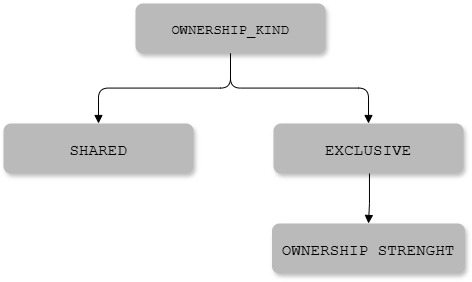
\includegraphics[width=10cm, keepaspectratio]{img/Policy QoS DDS_2.jpg}
    \caption{Illustrazione policy QoS del DDS}\label{Mappa QoS}
\end{figure}
% AFTER si potrebbe fare nei capitoli introduttivi una mappa che racchiuda
% i tipi di variabili che usano i QoS (int, double,.. etc) per i capitoli
% che spiegano meglio i concetti introduttivi


Questo attacco é possibile solo se certe policy QoS vengono
modificate durante l'esecuzione della rete, specialmente il parametro
OWNERSHIP-KIND che gestisce quanti DataWriter possono scrivere per un
determinato topic. Una descrizione accurata di altre policy QoS viene 
effettuata nella sottosezione~\ref{Le policy QoS nel dettaglio}.
Questo parametro può essere impostato in due modi diversi:
\begin{itemize}
    \item SHARED: in questo modo più di un DataWriter possono aggiornare le
    informazioni di un topic. Inoltre un DataReader si può iscrivere a
    qualsiasi scrittore dello stesso topic.
    \item EXCLUSIVE: solo un DataWriter può aggiornare le informazioni di un
    topic. Il DataWriter che ha il permesso di scrittura per il topic è quello
    che dispone di un OWNERSHIP-strength con valore più alto.
\end{itemize}
% https://www.omgwiki.org/ddsf/doku.php?id=ddsf:public:guidebook:06_append:02_quality_of_service:ownership
% https://www.omgwiki.org/ddsf/doku.php?id=ddsf:public:guidebook:06_append:02_quality_of_service:ownership_strength
In una rete dove si utilizza un OWNERSHIP-kind di tipo EXCLUSIVE è possibile
utilizzare l'OWNERSHIP-strength a favore
dell'attaccante. Infatti è possibile far ricevere informazioni a un DataWriter
in maniera errata, dato che quest'ultimo non riceverà più informazioni da
una fonte affidabile 
\cite{DBLP:conf/malware/MichaudDL18}.


\subsection{Dettagli attacco}
L'attaccante, con un DataWriter in suo possesso all'interno di una rete DDS,
può sfruttare il fatto che il topic preso di mira può essere aggiornato
solo dal DataWriter con l'OWNERSHIP-strength più alta.
Per effettuare questo attacco, tutto quello che serve, è sapere il topic che
si vuole modificare, le policy QoS in uso e il valore dell ownership-strength.
L'ultimo passo è quello di impostare il topic scelto nel DataWriter
dell'attaccante con OWNERSHIP-strength superiore a quello utilizzato dal
DataWriter originario.
Ora i DataReader che sono iscritti al topic bersaglio
ricevono le informazioni dal DataWriter dell'attaccante
\cite{DBLP:conf/malware/MichaudDL18}.


\subsection{Conclusioni}
L'OWNERSHIP-kind di tipo EXCLUSIVE è utilizzata in contesti dove le
informazioni ricevute dal DataReader devono essere accurate dato che un singolo
scrittore (in molti casi si tratta di un sensore) può mandare nuovi aggiornamenti
del topic. Se l'attaccante, dovesse riuscire a modificare i valori del topic con
questo attacco, potrebbe causare molti danni,
specialmente se il DataWriter dell'attaccante riesce a mandare degli aggiornamenti
al topic senza essere scoperto
\cite{DBLP:conf/malware/MichaudDL18}.

Una soluzione utile per mitigare questo attacco potrebbe essere l'utilizzo
dell'estensione DDS security. Utilizzando i plugin relativi al controllo accesso,
come illustrato nella sottosezione~ref{Access Control Service Plugin}, permette
di evitare che un attaccante possa modificare le policy QoS come 
l'OWNERSHIP-strength.


\section{Modifica maligna di LIFESPAN QoS}

Un'altra policy QoS che può essere usata come vettore di attacco è quella
che regola il parametro LIFESPAN. Questa regola corrisponde al tempo limite massimo 
di validitá per la
lettura di pacchetti da parte di un DataReader. Per determinare se un pacchetto
di un determinato topic è scaduto viene utilizzato il timestamp di creazione
aggiungendo il LIFESPAN impostato; se questo expiration time risulta
superiore all'orario durante la ricezione del DataReader, allora il pacchetto
ricevuto è ancora valido. 
Per funzionare gli orologi del DataWriter e del DataReader
devono essere sincronizzati tra di loro.

Un'altra policy da considerare è quella riguardo all'affidabilità
(RELIABILITY) dei dati riguardanti un topic che può essere impostata in due
modi:
\begin{itemize}
    \item RELIABLE: questa impostazione costringe il DataReader a farsi
    ritrasmettere dal DataWriter i pacchetti mancanti o ricevuti in maniera errata.
    In questo modo le informazioni del DataReader saranno sempre corrette anche
    se non sempre saranno aggiornate in tempo reale.
    \item BEST-EFFORT: l'impostazione predefinita non consente il recupero
    dei pacchetti mancanti o corrotti
    del DataReader, quindi, quest'ultimo potrebbe anche perdere dei pacchetti 
    che gli sono stati inviati \cite{dds1.4}.
\end{itemize}
% https://www.omgwiki.org/ddsf/doku.php?id=ddsf:public:guidebook:06_append:02_quality_of_service:reliability
Se il LIFESPAN dei pacchetti, contenenti i dati del topic,
viene impostato con valori molto piccoli, si verificheranno problemi di comunicazione
tra DataWriter e DataReader, dato che non sará possbile effettuare la lettura di 
certi pacchetti inviati. Impostando il valore RELIABLE tra le policy QoS di
RELIABILITY é possibile mitigare 
solo parzialmente questa vulnerabilitá
\cite{DBLP:conf/malware/MichaudDL18}.

% https://www.omgwiki.org/ddsf/doku.php?id=ddsf:public:guidebook:06_append:02_quality_of_service:lifespan


\subsection{Dettagli attacco}
Avendo sotto controllo i parametri LIFESPAN e RELIABLE, l'attaccante può modificare le
policy dei DataWriter in modo tale da avere il LIFESPAN molto piccolo. Così
facendo, i pacchetti spediti dal publisher arriveranno già scaduti al DataReader,
rendendoli inutilizzabili. In certi casi il pacchetto che deve essere inviato
viene distrutto dallo stesso DataWriter all'interno della sua coda prima dell'invio. 
In questo questa vulnerabilità è stato verificata impostando il valore di
LIFESPAN < 80ms dove si è visto che nessun pacchetto raggiunge il DataReader.
Se si aumenta il valore tra gli 80ms e i 100ms già si può notare che dei pacchetti
vengono letti con successo dal DataReader, mentre altri vengono eliminati prima
della lettura. Infine impostando un valore LIFESPAN >= 120ms si può notare che
la comunicazione tra publisher e subscriber avviene senza nessun problema.

Un dettaglio da aggiungere è che se si imposta la policy
dell'affidabilità (RELIABILITY) con valore RELIABLE, i millisecondi utilizzati
dal LIFESPAN per compromettere le comunicazioni tra DataReader e DataWriter
devono essere moltiplicati per un fattore di 0.01. Quindi, ad esempio se si
ottiene un completo annullamento delle comunicazioni con un LIFESPAN < 80ms
utilizzando il la RELIABILITY di tipo BEST-EFFORT, per ottenere lo stesso
risultato con RELIABILITY di tipo RELIABLE dobbiamo impostare un
LIFESPAN < 0.8ms
\cite{DBLP:conf/malware/MichaudDL18}.

\subsection{Conclusioni}
Questo test è stato dimostrato con RTI Shapes Demo che 
implementa una
soluzione DDS di RTI corrispondente alle specifiche dello standard OMG.
Inizialmente molte reti DDS hanno impostato la RELIABILITY
di tipo BEST-EFFORT che è l'impostazione predefinita. Quindi nella maggior parte
dei casi l'attaccante non si deve preoccupare di modificare questo parametro.

Una possibile soluzione sarebbe quella di impostare qualche tipo di controllo
in modo tale da avvertire un operatore umano se molti pacchetti vengono
scartati perché arrivati con un LIFESPAN scaduto. Questo controllo potrebbe
essere anche utile, nel caso in cui il DataWriter e il DataReader si trovassero
distanti fisicamente tra di loro, per verificare la qualità del collegamento
\cite{DBLP:conf/malware/MichaudDL18}.



% Definizione di un colore personalizzato
\definecolor{customgray}{rgb}{0.70, 0.70, 0.70} % Grigio chiaro

% Regolazione dello spessore delle linee
\setlength{\arrayrulewidth}{1.0pt} % Spessore linee generali
% \renewcommand{\arraystretch}{1.2} % Altezza righe


\begin{table}[H]
    \centering
    \rowcolors{2}{black!5}{white}
    \resizebox{\linewidth}{!}{%
        \begin{tabular}{|c|c|c|c|c|c|}
            \hline
            \rowcolor{customgray}
            \multicolumn{1}{|>{\columncolor{customgray}}c|}{\tabularCenterstack{c}{\textbf{Tipo di}\\ \textbf{attacco}}} &
            \multicolumn{1}{>{\columncolor{customgray}}c|}{\tabularCenterstack{c}{\textbf{Vettore} \\ \textbf{attacco}}} &
            \multicolumn{1}{>{\columncolor{customgray}}c|}{\tabularCenterstack{c}{\textbf{Protoc.}/ \\ \textbf{Estens.}}} &
            \multicolumn{1}{>{\columncolor{customgray}}c|}{\tabularCenterstack{c}{\textbf{Bersaglio} \\ \textbf{nella rete}}} &
            \multicolumn{1}{>{\columncolor{customgray}}c|}{\tabularCenterstack{c}{\textbf{Software}}} &
            \multicolumn{1}{>{\columncolor{customgray}}c|}{\tabularCenterstack{c}{\textbf{Soluzione}}} \\
            \hline
            \tabularCenterstack{c}{Discovery \\ devices \cite{White2017AnII}} &
            \tabularCenterstack{c}{Verbose nature \\ of RTPS} &
            \tabularCenterstack{c}{DDSI-RTPS} &
            \tabularCenterstack{c}{Tutti i par-\\tecipanti} &
            \tabularCenterstack{c}{Sniffer \\ python} &
            \tabularCenterstack{c}{WireGuard} \\
            \specialrule{0.3pt}{0pt}{0pt} % Linea più spessa dopo l'intestazione
            \tabularCenterstack{c}{DDos \cite{White2017AnII}} &
            \tabularCenterstack{c}{Heartbeat \\ sequence number} &
            \tabularCenterstack{c}{DDSI-RTPS} &
            \tabularCenterstack{c}{DataReader} &
            \tabularCenterstack{c}{Sniffer \\ python} &
            \tabularCenterstack{c}{-} \\
            \specialrule{0.3pt}{0pt}{0pt} % Linea più spessa dopo l'intestazione
            \tabularCenterstack{c}{DDoS \cite{DBLP:conf/asiaccs/WangLG24}} &
            \tabularCenterstack{c}{Authentication \\ challenge} &
            \tabularCenterstack{c}{DDS security 1.1 \\ Discovery protoc.} &
            \tabularCenterstack{c}{Tutti i par-\\tecipanti} &
            \tabularCenterstack{c}{Proverif} &
            \tabularCenterstack{c}{Scadenza richieste \\ di autenticazione} \\
            \specialrule{0.3pt}{0pt}{0pt} % Linea più spessa dopo l'intestazione
            \tabularCenterstack{c}{QoS policy \cite{DBLP:conf/malware/MichaudDL18}} &
            \tabularCenterstack{c}{ownership-strength} &
            \tabularCenterstack{c}{DDSI-RTPS} &
            \tabularCenterstack{c}{DataReader} &
            \tabularCenterstack{c}{RTI \\ shapes} &
            \tabularCenterstack{c}{DDS security: \\ Access Control} \\
            \specialrule{0.3pt}{0pt}{0pt} % Linea più spessa dopo l'intestazione
            \tabularCenterstack{c}{QoS policy \cite{DBLP:conf/malware/MichaudDL18}} &
            \tabularCenterstack{c}{LIFESPAN} &
            \tabularCenterstack{c}{DDSI-RTPS} &
            \tabularCenterstack{c}{DataReader} &
            \tabularCenterstack{c}{RTI \\ shapes} &
            \tabularCenterstack{c}{Controllo per \\ LIFESPAN scartati} \\
            \specialrule{0.3pt}{0pt}{0pt} % Linea più spessa dopo l'intestazione
            
            % Aggiungere altre linee

            \hline
        \end{tabular}
        }
        \caption{La versione DDS in tutti i casi è la 1.4}
    \end{table}








    %\chapter{Vulnerabilità standard DDS}


In questo capitolo ci occuperemo di analizzare e comprendere delle vulnerabilità
del middleware DDS standard OMG (Object Management Group) \cite{8469351}. 
In particolare
verrà analizzato il vettore d'attacco, il protocollo utilizzato, il bersaglio
dell'attacco e infine verrà proposta una soluzione applicabile per
mitigare i possibili attacchi. %  Nel prossimo capitolo grazie all'aiuto
% del software --inserire software-- riusciremo a capire come queste vulnerabilità
% possono essere ricreate in un ambiente simulato.
Queste vulnerabilità in molti casi, possono essere sfruttate 
quando un partecipante del domain DDS è sotto il controllo di un attaccante
o quando è possibile modificare i file di configurazione delle policy QoS 
del domain.

Queste vulnerabilità riguardano la versione del DDS 1.4 con le specifiche 
dello standard OMG.

Nella Tabella~\ref{tabvulndds} viene mostrato un riassunto di tutte
le vulnerabilità mostrate in questo capitolo. Come si può notare dai dati 
la soluzione più efficace per mitigare questi attacchi è utilizzare 
l'estensione DDS security che permette di crittografare le varie comunicazioni
scambiate tra le varie entità, rendendo più difficile per un attore 
malevolo
analizzare i contenuti dei pacchetti.






% Definizione di un colore personalizzato
\definecolor{customgray}{rgb}{0.70, 0.70, 0.70} % Grigio chiaro

% Regolazione dello spessore delle linee
\setlength{\arrayrulewidth}{1.0pt} % Spessore linee generali
% \renewcommand{\arraystretch}{1.2} % Altezza righe


\begin{table}[H]
    \centering
    \rowcolors{2}{black!5}{white}
    \resizebox{\linewidth}{!}{%
        \begin{tabular}{|c|c|c|c|c|c|}
            \hline
            \rowcolor{customgray}
            \multicolumn{1}{|>{\columncolor{customgray}}c|}{\tabularCenterstack{c}{\textbf{Tipo di}\\ \textbf{attacco}}} &
            \multicolumn{1}{>{\columncolor{customgray}}c|}{\tabularCenterstack{c}{\textbf{Vettore} \\ \textbf{attacco}}} &
            \multicolumn{1}{>{\columncolor{customgray}}c|}{\tabularCenterstack{c}{\textbf{Protoc.}/ \\ \textbf{Estens.}}} &
            \multicolumn{1}{>{\columncolor{customgray}}c|}{\tabularCenterstack{c}{\textbf{Bersaglio} \\ \textbf{nella rete}}} &
            \multicolumn{1}{>{\columncolor{customgray}}c|}{\tabularCenterstack{c}{\textbf{Software}}} &
            \multicolumn{1}{>{\columncolor{customgray}}c|}{\tabularCenterstack{c}{\textbf{Soluzione}}} \\
            \hline
            \tabularCenterstack{c}{Discovery \\ devices \cite{White2017AnII}} &
            \tabularCenterstack{c}{Verbose nature \\ of RTPS} &
            \tabularCenterstack{c}{RTPS-SDPD} &
            \tabularCenterstack{c}{Tutti i par-\\tecipanti} &
            \tabularCenterstack{c}{Sniffer \\ Python} &
            \tabularCenterstack{c}{DDS security/ \\ WireGuard} \\
            \specialrule{0.3pt}{0pt}{0pt} % Linea più spessa dopo l'intestazione
            \tabularCenterstack{c}{DDos \cite{White2017AnII}} &
            \tabularCenterstack{c}{Heartbeat \\ sequence number} &
            \tabularCenterstack{c}{RTPS} &
            \tabularCenterstack{c}{DataReader} &
            \tabularCenterstack{c}{Sniffer \\ Python} &
            \tabularCenterstack{c}{DDS security: \\ Auth Control} \\
            \specialrule{0.3pt}{0pt}{0pt} % Linea più spessa dopo l'intestazione
            \tabularCenterstack{c}{DDoS \cite{DBLP:conf/asiaccs/WangLG24}} &
            \tabularCenterstack{c}{Authentication \\ challenge} &
            \tabularCenterstack{c}{DDS security 1.1 \\ Discovery protoc.} &
            \tabularCenterstack{c}{Tutti i par-\\tecipanti} &
            \tabularCenterstack{c}{Proverif} &
            \tabularCenterstack{c}{Scadenza richieste \\ di autenticazione} \\
            \specialrule{0.3pt}{0pt}{0pt} % Linea più spessa dopo l'intestazione
            \tabularCenterstack{c}{QoS policy \cite{DBLP:conf/malware/MichaudDL18}} &
            \tabularCenterstack{c}{Policy: \\ Ownership} &
            \tabularCenterstack{c}{RTPS} &
            \tabularCenterstack{c}{DataReader} &
            \tabularCenterstack{c}{RTI \\ shapes} &
            \tabularCenterstack{c}{DDS security: \\ Access Control} \\
            \specialrule{0.3pt}{0pt}{0pt} % Linea più spessa dopo l'intestazione
            \tabularCenterstack{c}{QoS policy \cite{DBLP:conf/malware/MichaudDL18}} &
            \tabularCenterstack{c}{Policy: \\ Lifespan} &
            \tabularCenterstack{c}{RTPS} &
            \tabularCenterstack{c}{DataReader} &
            \tabularCenterstack{c}{RTI \\ shapes} &
            \tabularCenterstack{c}{Controllo per \\ Lifespan scartati} \\
            % \specialrule{0.3pt}{0pt}{0pt} % Linea più spessa dopo l'intestazione
            
            % Aggiungere altre linee

            \hline
        \end{tabular}
        }
        \caption{Riassunto delle vulnerabilità del DDS analizzate.}
        \label{tabvulndds}
    \end{table}




\section{Blocco DataReader tramite sequence number}

%\subsubsection{Prologo}
Il vettore di attacco si trova nel messages module del protocollo RTPS
descritto nella Sezione~\ref{Messages module}. Questo modulo
si occupa di scambiare messaggi tra i DataReader e i DataWriter 
all'interno un domain DDS.

Per effettuare questi scambi di messaggi vengono utilizzati dei sottomessaggi,
in particolare l'HEARTBEAT e l'ACKNACK.
L'HEARTBEAT contiene al suo interno il sequence number che tiene traccia 
del numero di aggiornamenti di un topic da parte di DataWriter, mentre
l'ACKNACK inviato da un DataReader
serve per confermare al DataWriter la ricezione di nuovi dati 
riguardo un topic.
Quando il DataReader riceve il sequence number all'interno di un HEARTBEAT
può identificare se ci sono o no dei pacchetti mancanti e in caso segnalarli al
DataWriter \cite{White2017AnII}.
Inoltre se il parametro FINAL è attivo in un sottomessaggio HEARTBEAT, il DataReader 
deve sempre rispondere al DataWriter con ACKNACK dopo aver ricevuto nuovi aggiornamenti.
Il DataWriter, nel frattempo, rimarrà in attesa del sottomessaggio 
ACKNACK prima di 
inviare nuovi aggiornamenti al DataReader.
Questo sistema aiuta il DataReader a rimanere sempre sincronizzato con il 
DataWriter.

I controlli del sequence number all'interno dell'HEARTBEAT 
non sono sufficienti per mitigare questo attacco:
\begin{itemize}
    \item Un primo controllo viene effettuato per verificare che non ci siano 
    valori negativi;
    \item Un altro controllo serve a determinare se l'ultimo sequence number
    appena ricevuto ha un valore minore rispetto a quello ricevuto in precedenza
    \cite{White2017AnII};
\end{itemize}


\subsection{Dettagli attacco e conclusioni}

Per sfruttare questa vulnerabilità l'attaccante deve utilizzare qualche 
strumento per sniffare la comunicazione tra il DataReader e il DataWriter,
intercettando i
sottomessaggi HEARTBEAT. Dopo aver catturato un HEARTBEAT diretto verso 
un DataReader e modificato 
il suo sequence number assegnandogli un valore molto alto, 
l'attaccante lo rinvia al suo destinatario originario.
Una volta ricevuto il sottomessaggio il DataReader si metterà quindi 
in attesa di un HEARTBEAT con un sequence number 
superiore a quello appena ricevuto. Di conseguenza il DataReader
non elaborerà più i messaggi legittimi mandati dal DataWriter,
dato che hanno sequence number più piccoli.
Solo un messaggio HEARTBEAT con un sequence number
maggiore a quello del DataReader farà ripristinare la sua esecuzione 
\cite{White2017AnII}.


% \subsection{Conclusioni}z
Di solito questo tipo di attacco è difficile da identificare. 
Un messaggio HEARTBEAT riguarda un solo topic, quindi il resto delle
comunicazioni che avvengono su topic differenti o anche sullo stesso 
topic, ma con un DataReader diverso, non subiranno cambiamenti.
Questa vulnerabilità può essere mitigata utilizzando l'estensione
DDS security in modo tale da crittografare i messaggi e rendere 
impossibile per l'attaccante effettuare modifiche al 
sequence number. 


\section{DDoS sfruttando estensione DDS security}
Questo vettore di attacco si trova nell'estensione del DDS chiamata
DDS security, descritto nella Sezione~\ref{DDS Security}; 
in particolare la versione utilizzata è la versione 1.1.
Il DDS security si occupa di stabilire una
connessione sicura tra i vari dispositivi della rete, utilizzando 
dei plugin per effettuare: autenticazione, controllo accesso, crittografia,
login e data logging \cite{ddssecurity1.1}.

Ogni partecipante del domain DDS deve essere autenticato reciprocamente
dalle altre entità appartenenti allo stesso domain.
Successivamente due entità,
per iniziare una comunicare tra di loro, devono prima
scambiarsi le chiavi private
in modo
sicuro tramite protocollo Diffie-Hellman in modo tale da poter 
crittare i successivi
messaggi. Nell'utilizzo di Diffie-Hellman vengono utilizzate
le challenge (Sezione ~\ref{Processo di autenticazione}), 
che corrispondono a valori che variano nel tempo, 
inseriti durante il calcolo
della firma digitale richiesta dal protocollo. 
Queste challenge vengono utilizzate per rendere le varie sessioni 
di autenticazione uniche evitando così attacchi di tipo replay
\cite{DBLP:conf/asiaccs/WangLG24}.

% controllare sta robbba


\subsection{Dettagli attacco e conclusioni}
L'attacco DDoS avviene durante la fase di autenticazione del
DDS security 1.1, in particolare quando un nuovo dispositivo tenta di
collegarsi alla rete e manda una richiesta di autenticazione
all'entità con cui vuole aprire una comunicazione. 
La richiesta del partecipante viene intercettata
dall'attaccante che modifica i valori della challenge crittografica 
all'interno del pacchetto. Modificando ripetutamente questi valori, l'attaccante
inizia a inviare molteplici richieste crittografiche alla sua vittima.
Il partecipante così comincerà a calcolare le firme digitali per effettuare
l'autenticazione, consumando tutte le sue risorse.
Dato che, la vittima è probabilmente un dispositivo IoT
(Internet of Things)
che non dispone di una potenza di calcolo molto elevata, si ritroverà
occupata per tutto il tempo necessario a calcolare diverse firme digitali
ricevute dall'attaccante, bloccando così il suo funzionamento
\cite{DBLP:conf/asiaccs/WangLG24}.


% \subsection{Conclusioni}
Questo attacco è stato scoperto con Proverif, un tool che viene usato
per individuare vulnerabilità nei protocolli crittografici. 
È stato utilizzato in molti studi, ad esempio nell'analisi della 
posta elettronica certificata e nell'analisi del TLS 1.3 \cite{proverifmanual}.
% https://bblanche.gitlabpages.inria.fr/proverif/manual.pdf

Una raccomandazione per mitigare questo attacco è quello di cambiare delle
policy QoS impostando un tempo limite massimo per effettuare
l'autenticazione. Queste policy possono fare in modo
che i partecipanti non si trovino sopraffatti dalle troppe richieste di
autenticazione. Un allarme potrebbe essere utile per identificare possibili
tentativi DDoS di questo tipo, allertando così un amministratore
\cite{DBLP:conf/asiaccs/WangLG24}.


\section{Enumeration sniff}
% Devo spiegare il modulo discovery
Prendendo in considerazione, il protocollo RTPS,
descritto nella Sezione~\ref{Discovery module}, e il suo modulo discovery,
possiamo notare che di default i messaggi sono molto verbose, 
scambiando le informazioni in
chiaro durante le comunicazioni tra i vari partecipanti \cite{White2017AnII}.
Il modulo 
discovery del protocollo RTPS a sua volta si suddivide in
altri 2 protocolli, che sono necessari per le specifiche DDS:
% (foglio 5 pag 123)
\begin{itemize}
    \item Simple Participant Discovery Protocol (SPDP).
    \item Simple Endpoint Discovery Protocol (SEDP).
\end{itemize}



\subsection{Dettagli attacco e coclusioni}
Per questo attacco ci focalizzeremo in particolare sull'SPDP che serve ad
individuare la presenza dei partecipanti al resto delle
entità nel domain. In particolar modo
il funzionamento si basa su un messaggi di tipo multicast che vengono
mandati a tutti i dispositivi riguardo ai partecipanti attivi
% (foglio 5 pag 125)
\cite{ddsrtps}.

L'attaccante sniffando questi messaggi (all'interno di un domain DDS)
di tipo multicast RTPS-SPDP,
utilizzando anche un semplice script Python, infatti potrà 
vedere il loro contenuto in maniera chiara.

All'interno di un pacchetto di questo tipo possiamo trovare:
l'indirizzo IP dell'host, il prefisso GUID dell'RTPS,
la versione dellRTPS, l'ID del venditore, metadati 
riguardanti la sincronizzazione
ed infine il contenuto dei sottomessaggi \cite{White2017AnII}.


% \subsection{Conclusioni}
Fare una ricognizione della rete DDS senza effettuare veri e propri
attacchi di tipo attivo può essere molto utile per un attaccante che 
ha il compito di penetrare in modo attivo
una rete DDS. In molti casi tutto quello che deve fare l'attaccante
è osservare i messaggi che vengono scambiati all'interno del network.
Successivamente quando si ottengono informazioni a sufficienza sarà più
facile per l'attaccante trovare altre vulnerabilità
\cite{White2017AnII}.

Di solito questo tipo di attacco è difficile da identificare e possono essere
effettuati senza lasciare tracce di nessun tipo, dato che l'attaccante non 
manda pacchetti.
Una soluzione potrebbe essere usare l'estensione DDS security o 
eseguire la connessione tra i nodi tramite un tunnel con WireGuard per crittare
le comunicazioni.






% \begin{figure}[H]
%     \centering
%     \includesvg[width=15cm,keepaspectratio]{img/Policy QoS DDS.drawio.svg}
%     \caption{Illustrazione policy QoS del DDS}\label{Mappa QoS svg}
% \end{figure}






\section{Modifica maligna OWNERSHIP\_STRENGTH}

\begin{figure}[H]
    \centering
    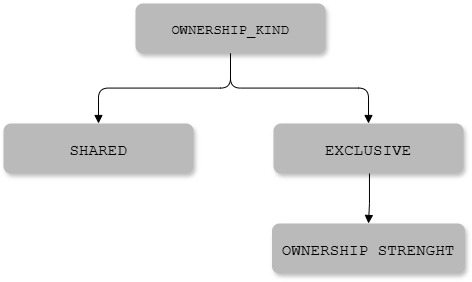
\includegraphics[width=10cm, keepaspectratio]{img/Policy QoS DDS_2.jpg}
    \caption{Illustrazione policy QoS del DDS}\label{Mappa QoS}
\end{figure}
\label{img/Policy QoS DDS_2}
% AFTER si potrebbe fare nei capitoli introduttivi una mappa che racchiuda
% i tipi di variabili che usano i QoS (int, double,.. etc) per i capitoli
% che spiegano meglio i concetti introduttivi


Questo attacco è realizzabile solo se certe policy QoS vengono
modificate durante l'esecuzione della rete, specialmente il parametro
OWNERSHIP-KIND che gestisce quanti DataWriter possono scrivere per un
determinato topic. Una descrizione accurata di altre policy QoS viene 
effettuata nella Sezione~\ref{Le policy QoS nel dettaglio}.
Questo parametro può essere impostato in due modi diversi:
\begin{itemize}
    \item SHARED: in questo modo più di un DataWriter possono aggiornare le
    informazioni di un topic.
    \item EXCLUSIVE: solo un DataWriter può aggiornare le informazioni di un
    topic. Il DataWriter che ha il permesso di scrittura per il topic è quello
    che dispone di un OWNERSHIP-strength con valore più alto.
\end{itemize}
% https://www.omgwiki.org/ddsf/doku.php?id=ddsf:public:guidebook:06_append:02_quality_of_service:ownership
% https://www.omgwiki.org/ddsf/doku.php?id=ddsf:public:guidebook:06_append:02_quality_of_service:ownership_strength
Nella Figura~\ref{img/Policy QoS DDS_2} viene proposto uno schema riassuntivo
delle policy QoS relative a questo attacco.
In una rete dove si utilizza un OWNERSHIP-kind di tipo EXCLUSIVE è consente
all'attaccante di utilizzare l'OWNERSHIP-strength a suo favore.
Infatti è possibile far ricevere informazioni a un DataWriter
in maniera errata, dato che quest'ultimo non riceverà più dati da
una fonte affidabile 
\cite{DBLP:conf/malware/MichaudDL18}.


\subsection{Dettagli attacco e conclusioni}
L'attaccante, con un DataWriter in suo possesso all'interno di una rete DDS,
può sfruttare il fatto che il topic preso di mira può essere aggiornato
solo dal DataWriter con l'OWNERSHIP-strength più alta.
Per effettuare questo attacco, tutto quello che serve, è 
essere a conoscenza del topic che
si vuole modificare, le policy QoS in uso e il valore dell OWNERSHIP-strength.
L'ultimo passo è quello di impostare la policy QoS nel DataWriter
dell'attaccante con OWNERSHIP-strength superiore a quello utilizzato dal
DataWriter originario.
Ora i DataReader che sono iscritti al topic bersaglio
ricevono dati dal DataWriter dell'attaccante
\cite{DBLP:conf/malware/MichaudDL18}.


% \subsection{Conclusioni}
Questa vulnerabilità è stata analizzata con l'ausilio di RTI Shapes Demo, un 
software che emula una rete DDS corrispondente alle specifiche 
dello standard OMG, sviluppato da Real-Time Innovations (RTI).

L'OWNERSHIP-kind di tipo EXCLUSIVE è utilizzata in contesti dove le
informazioni ricevute dal DataReader devono essere accurate dato che un singolo
DataWriter (in molti casi si tratta di un sensore) può mandare nuovi aggiornamenti
del topic. Se l'attaccante, dovesse riuscire a modificare i valori del topic con
questo attacco, potrebbe causare molti danni,
specialmente se il DataWriter dell'attaccante riesce a mandare degli aggiornamenti
al topic senza essere scoperto
\cite{DBLP:conf/malware/MichaudDL18}.

Una soluzione utile per mitigare questo attacco potrebbe essere l'utilizzo
dell'estensione DDS security. Utilizzando i plugin relativi al controllo accesso,
come illustrato nella Sezione~\ref{AccessControlServicePlugin}, permette
di evitare che un attaccante possa modificare le policy QoS inclusa 
l'OWNERSHIP-strength.


\section{Modifica maligna di LIFESPAN QoS}

Un'altra policy QoS che può essere usata come vettore di attacco è quella
che regola il parametro LIFESPAN. Questa regola corrisponde al tempo limite massimo 
di validità per la
lettura di pacchetti da parte di un DataReader. Per determinare se un pacchetto
di un determinato topic è scaduto viene utilizzato il timestamp di creazione
aggiungendo il LIFESPAN impostato; se questo risultato chiamato 
expiration time risulta
superiore all'orario durante la ricezione del DataReader, allora il pacchetto
ricevuto è ancora valido. 
Per funzionare gli orologi interni del DataWriter e del DataReader
devono essere sincronizzati tra di loro.

Un'altra policy da considerare è quella riguardo all'affidabilità
(RELIABILITY) dei dati riguardanti un topic che può essere impostata in due
modi:
\begin{itemize}
    \item RELIABLE: questa impostazione costringe il DataReader a farsi
    ritrasmettere dal DataWriter i pacchetti mancanti o ricevuti in maniera errata.
    In questo modo le informazioni del DataReader saranno sempre corrette anche
    se non sempre saranno aggiornate in tempo reale.
    \item BEST-EFFORT: l'impostazione predefinita non consente il recupero
    dei pacchetti mancanti o corrotti
    del DataReader, quindi, quest'ultimo potrebbe anche perdere dei pacchetti 
    che gli sono stati inviati \cite{dds1.4}.
\end{itemize}
% https://www.omgwiki.org/ddsf/doku.php?id=ddsf:public:guidebook:06_append:02_quality_of_service:reliability
Se il LIFESPAN dei pacchetti, contenenti i dati del topic,
viene impostato con valori molto piccoli, si verificheranno problemi di comunicazione
tra DataWriter e DataReader, dato che non sarà possibile effettuare la lettura di 
certi pacchetti inviati. Impostando il valore RELIABLE tra le policy QoS con
RELIABILITY è possibile mitigare 
solo parzialmente questa vulnerabilità
\cite{DBLP:conf/malware/MichaudDL18}.

% https://www.omgwiki.org/ddsf/doku.php?id=ddsf:public:guidebook:06_append:02_quality_of_service:lifespan


\subsection{Dettagli attacco e conclusioni}
Avendo sotto controllo i parametri LIFESPAN e RELIABLE, l'attaccante modificherà le
policy dei DataWriter in modo tale da avere il LIFESPAN molto piccolo. Così
facendo, i pacchetti spediti dal publisher arriveranno già scaduti al DataReader,
rendendoli inutilizzabili. In certi casi il pacchetto che deve essere inviato
viene distrutto dallo stesso DataWriter all'interno della sua coda prima dell'invio. 
Questa vulnerabilità è stato verificata impostando il valore di
LIFESPAN < 80ms dove si è visto che nessun pacchetto raggiunge il DataReader.
Se si aumenta il valore tra gli 80ms e i 100ms già si può notare che dei pacchetti
vengono letti con successo dal DataReader, mentre altri vengono eliminati prima
della lettura. Infine impostando un valore LIFESPAN >= 120ms si può notare che
la comunicazione tra publisher e subscriber avviene senza nessun problema.

Un dettaglio da aggiungere è che se si imposta la policy
dell'affidabilità (RELIABILITY) con valore RELIABLE, i millisecondi necessari
del LIFESPAN per compromettere le comunicazioni tra DataReader e DataWriter
devono essere moltiplicati per un fattore di 0.01. Quindi, ad esempio se si
ottiene un completo annullamento delle comunicazioni con un LIFESPAN < 80ms
utilizzando il la RELIABILITY di tipo BEST-EFFORT, per ottenere lo stesso
risultato con RELIABILITY di tipo RELIABLE dobbiamo impostare un
LIFESPAN < 0.8ms
\cite{DBLP:conf/malware/MichaudDL18}.

% \subsection{Conclusioni}
Anche questo test è stato dimostrato con RTI Shapes Demo che 
implementa una
soluzione DDS di RTI corrispondente alle specifiche dello standard OMG.
Inizialmente molte reti DDS hanno impostato la RELIABILITY
di tipo BEST-EFFORT che è l'impostazione predefinita,
in modo tale da rendere possibili comunicazioni di tipo real-time.
Quindi nella maggior parte
dei casi l'attaccante non si deve preoccupare di modificare questo parametro.

Una possibile soluzione consiste nell'implementare qualche tipo di controllo
in modo tale da avvertire un operatore umano se molti pacchetti vengono
scartati perché arrivati con un LIFESPAN scaduto. Questo controllo potrebbe
essere anche utile, nel caso in cui il DataWriter e il DataReader si trovassero
distanti fisicamente tra di loro, per verificare la qualità del collegamento
\cite{DBLP:conf/malware/MichaudDL18}.



    % ...
    \input{conclusioni5}

    \bibliographystyle{plainnat}
    % Opzionale
    % \listoffigures
    % \listoftables
    \bibliography{bibliografia}

    \chapter*{Ringraziamenti}

Un sentito grazie ai miei genitori per il loro sostegno incondizionato, 
ai miei amici per avermi accompagnato in questo percorso con il loro supporto
e la loro compagnia, e alla mia ragazza per la pazienza
e l'incoraggiamento costante. Questa tesi è anche merito vostro.

\vspace{17mm}

\vs
\begin{flushright}
 Federico
\end{flushright}


    
\end{document}